\documentclass[border=3pt]{standalone}
% Shared preamble of the block diagrams: LaTeX fonts (Latin Modern, as in the thesis text) and TikZ styles.
% Compile with build.sh (needs pdflatex + TikZ). In the thesis, just include the compiled PDFs.
\usepackage[T1]{fontenc}
\usepackage{lmodern}
\usepackage{amsmath,amssymb,bm}
\usepackage{tikz}
\usetikzlibrary{arrows.meta,calc,fit,backgrounds}

\definecolor{boxblue}{RGB}{218,232,245}   \definecolor{edgeblue}{RGB}{143,180,220}
\definecolor{boxgreen}{RGB}{226,240,217}  \definecolor{edgegreen}{RGB}{140,190,120}
\definecolor{boxteal}{RGB}{213,238,240}   \definecolor{edgeteal}{RGB}{110,190,196}
\definecolor{boxpurple}{RGB}{232,224,243} \definecolor{edgepurple}{RGB}{170,140,205}
\definecolor{boxorange}{RGB}{252,228,214} \definecolor{edgeorange}{RGB}{240,160,115}
\definecolor{fwdc}{RGB}{62,106,153}       \definecolor{invc}{RGB}{232,98,44}
\definecolor{navy}{RGB}{31,58,95}         \definecolor{muted}{RGB}{90,100,115}

\tikzset{
  >=Stealth,
  icon/.style  ={draw=edgeblue, fill=boxblue, rounded corners=3pt, line width=0.6pt, minimum width=1.5cm, minimum height=1.15cm},
  block/.style ={draw=edgeblue, fill=boxblue, rounded corners=3pt, line width=0.6pt, align=center, text=navy, inner sep=4pt, font=\small},
  plain/.style ={draw=black, fill=white, rounded corners=3pt, line width=0.8pt, align=center, inner sep=4pt, font=\small},
  fwd/.style   ={-{Stealth[length=5pt,width=4pt]}, line width=0.9pt, color=fwdc},
  inv/.style   ={-{Stealth[length=5pt,width=4pt]}, line width=0.9pt, color=invc, dash pattern=on 3pt off 2pt},
  group/.style ={rounded corners=4pt, line width=0.9pt, dash pattern=on 4pt off 3pt},
  note/.style  ={font=\footnotesize, text=muted, align=center},
}
% plate icon: rectangle with resonator dots; #1 centre, #2 dots "x/y, x/y" in [-1,1]
\newcommand{\plateicon}[2]{\begin{scope}[shift={#1}]
  \draw[line width=0.7pt] (-0.55,-0.25) rectangle (0.55,0.25);
  \foreach \px/\py in {#2} {\fill (0.5*\px,0.19*\py) circle (1.7pt);}
\end{scope}}
% sketch of an ERP spectrum; #1 centre
\newcommand{\spectrumicon}[1]{\begin{scope}[shift={#1}]
  \draw[line width=0.6pt] (-0.55,0.42)--(-0.55,-0.40)--(0.55,-0.40);
  \draw[line width=0.85pt, line join=round, line cap=round] (-0.5,-0.32) -- (-0.3,-0.12) -- (-0.22,0.02) -- (-0.17,0.30) -- (-0.11,-0.02)
     -- (-0.02,0.14) -- (0.04,-0.08) -- (0.12,-0.02) -- (0.18,0.24) -- (0.24,-0.12) -- (0.38,0.0) -- (0.50,0.10);
\end{scope}}

\begin{document}
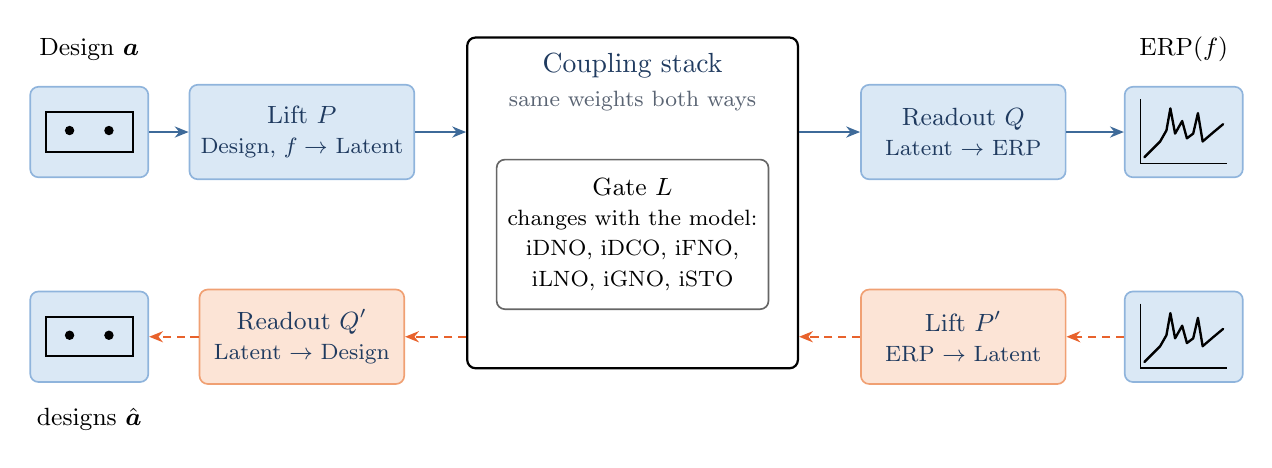
\begin{tikzpicture}
% forward row
\node[font=\small] at (0,3.05) {Design $\bm a$};
\node[icon] (d1) at (0,2.0) {}; \plateicon{(d1.center)}{-0.5/0.1, 0.5/0.1}
\node[block, minimum width=2.6cm, minimum height=1.2cm] (P) at (2.7,2.0) {Lift $P$\\ {\footnotesize Design, $f\to$ Latent}};
\node[block, minimum width=2.6cm, minimum height=1.2cm] (Q) at (11.1,2.0) {Readout $Q$\\ {\footnotesize Latent $\to$ ERP}};
\node[icon] (e1) at (13.9,2.0) {}; \spectrumicon{(e1.center)}
\node[font=\small] at (13.9,3.05) {ERP$(f)$};
% coupling stack with the gate
\node[plain, minimum width=4.2cm, minimum height=4.2cm, anchor=center] (stack) at (6.9,1.1) {};
\node[font=\normalsize, text=navy] at (6.9,2.85) {Coupling stack};
\node[note] at (6.9,2.4) {same weights both ways};
\node[plain, minimum width=3.3cm, minimum height=1.9cm, draw=black!60, line width=0.6pt] (gate) at (6.9,0.7)
   {Gate $L$\\ {\footnotesize changes with the model:}\\ {\footnotesize iDNO, iDCO, iFNO,}\\ {\footnotesize iLNO, iGNO, iSTO}};
% inverse row
\node[icon] (e2) at (13.9,-0.6) {}; \spectrumicon{(e2.center)}
\node[block, fill=boxorange, draw=edgeorange, minimum width=2.6cm, minimum height=1.2cm] (Pp) at (11.1,-0.6) {Lift $P'$\\ {\footnotesize ERP $\to$ Latent}};
\node[block, fill=boxorange, draw=edgeorange, minimum width=2.6cm, minimum height=1.2cm] (Qp) at (2.7,-0.6) {Readout $Q'$\\ {\footnotesize Latent $\to$ Design}};
\node[icon] (d2) at (0,-0.6) {}; \plateicon{(d2.center)}{-0.5/0.1, 0.5/0.1}
\node[font=\small] at (0,-1.65) {designs $\hat{\bm a}$};
\draw[fwd] (d1.east) -- (P.west);  \draw[fwd] (P.east) -- (stack.west |- P.east);
\draw[fwd] (stack.east |- Q.west) -- (Q.west);  \draw[fwd] (Q.east) -- (e1.west);
\draw[inv] (e2.west) -- (Pp.east);  \draw[inv] (Pp.west) -- (stack.east |- Pp.west);
\draw[inv] (stack.west |- Qp.east) -- (Qp.east);  \draw[inv] (Qp.west) -- (d2.east);
\end{tikzpicture}
\end{document}
